\section{Minimum Spanning Trees}\label{sec:2}

\subsection{Trees}\label{subsec:2.1}
A {\bf tree} is a connected acyclic graph; that is, a connected graph 
containing no cycles. 
\begin{center}
    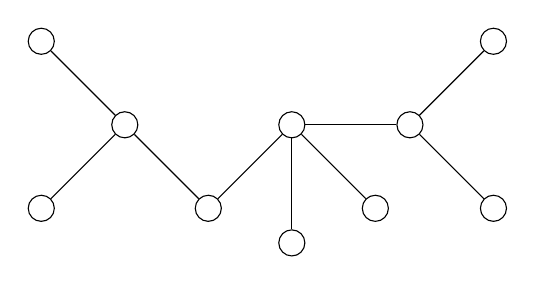
\begin{tikzpicture}[node distance={15mm}, main/.style = {draw, circle}] 
        \node[main] (1) {}; 
        \node[main] (2) [below right of=1] {};
        \node[main] (3) [below left of=2] {}; 
        \node[main] (4) [below right of=2] {};
        \node[main] (5) [above right of=4] {};
        \node[main] (6) [below of=5] {};
        \node[main] (7) [below right of=5] {};
        \node[main] (8) [right of=5] {};
        \node[main] (9) [above right of=8] {};
        \node[main] (10) [below right of=8] {};

        \draw (1) -- (2); \draw (2) -- (3); \draw (2) -- (4);
        \draw (4) -- (5); \draw (5) -- (6); \draw (5) -- (7);
        \draw (5) -- (8); \draw (8) -- (9); \draw (8) -- (10);
    \end{tikzpicture} 
\end{center}
\vspace{-0.25cm}
Given a graph $G = (V, E)$, a {\bf spanning tree} of $G$ is a graph $T = (V, F)$ 
such that $F \subseteq E$ and $T$ is a tree. We illustrate an example of a 
graph $G$ with a subtree $T$ using bold edges below. 
\begin{center}
    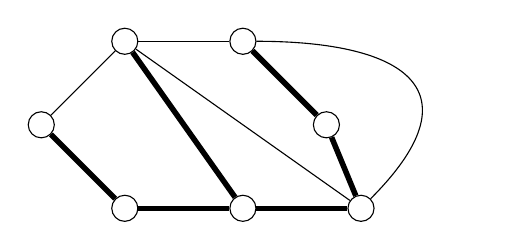
\begin{tikzpicture}[node distance={15mm}, main/.style = {draw, circle}] 
        \node[main] (1) {}; 
        \node[main] (2) [right of=1] {};
        \node[main] (3) [below left of=1] {}; 
        \node[main] (4) [below right of=2] {};
        \node[main] (5) [below right of=3] {};
        \node[main] (6) [right of=5] {};
        \node[main] (7) [right of=6] {};

        \draw (1) -- (2); 
        \draw (1) -- (3); 
        \draw [line width=2pt] (1) -- (6);
        \draw (1) -- (7);
        \draw [line width=2pt] (2) -- (4);
        \draw (2) to [out=0, in=45, looseness=2] (7);
        \draw [line width=2pt] (3) -- (5);
        \draw [line width=2pt] (4) -- (7);
        \draw [line width=2pt] (5) -- (6);
        \draw [line width=2pt] (6) -- (7);
    \end{tikzpicture} 
\end{center}
In an introductory graph theory course, such as MATH 239, 
it is shown that every tree on $n$ vertices has $n-1$ edges. The following 
theorem then gives us a useful characterization of trees. 

\begin{theo}{theo:2.1}
    Let $T = (V, F)$ be a graph. The following are equivalent:
    \begin{enumerate}[(i)]
        \item $T$ is a tree. 
        \item $T$ is connected and $|F| = |V| - 1$. 
        \item $T$ is acyclic and $|F| = |V| - 1$. 
    \end{enumerate}
\end{theo}

In particular, if we know that two of the conditions hold, then the 
third one is guaranteed.

\subsection{Minimum Spanning Trees}\label{subsec:2.2}
Given a connected graph $G = (V, E)$ and edge costs $c_e \geq 0$ for each 
$e \in E$, our goal is to find a spanning tree $T$ of minimum cost 
\[ c(T) := \sum_{e \in T} c_e. \] 
First, we'll set some notation. For a vertex $v \in V$, we define 
$\delta(v)$ to be the set of edges in $E$ incident to $v$. More generally, 
given a subset of vertices $S \subseteq V$, the {\bf cut induced by $S$} is 
defined to be the set 
\[ \delta(S) := \{uv \in E : u \in S,\, v \notin S\}. \] 
The following theorem will be extremely important for finding a minimum 
spanning tree. 

\begin{theo}{theo:2.2}
    Suppose that the costs $c_e \geq 0$ for $e \in E$ are distinct. 
    Let $S \subseteq V$ be such that $S \neq \varnothing$ and $S \neq V$, 
    and let 
    \[ e = \argmin_{f \in \delta(S)} c_f. \] 
    Then every minimum spanning tree contains the edge $e$. 
\end{theo}
